% F049: native TikZ/PGFPlots, computed from the stated mathematical model.
\begin{center}
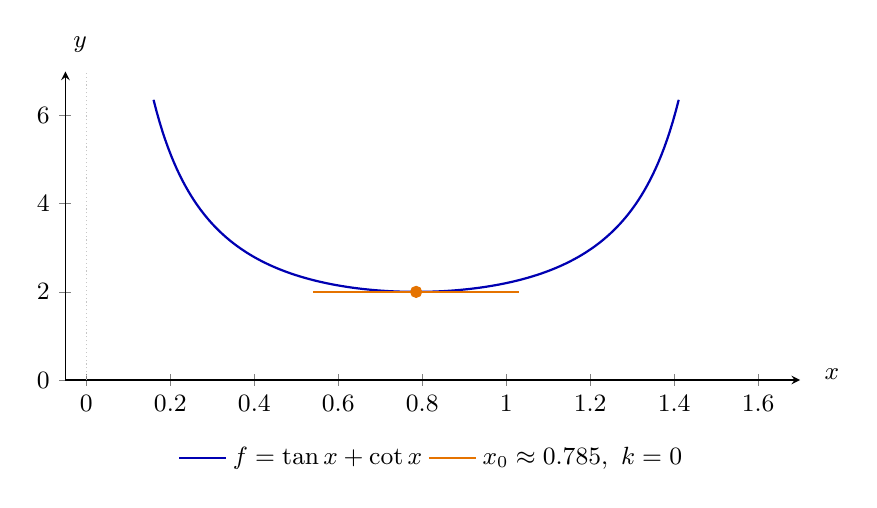
\begin{tikzpicture}[font=\small,>=stealth]
\begin{axis}[width=.90\linewidth,height=5.5cm,xmin=-0.05,xmax=1.7,ymin=0,ymax=7,
axis lines=left,xlabel={$x$},ylabel={$y$},font=\small,
xlabel style={at={(axis description cs:1.02,.02)},anchor=west},
ylabel style={rotate=-90,at={(axis description cs:.02,1.03)},anchor=south},
legend style={at={(axis description cs:.5,-.18)},anchor=north,draw=none,fill=none,font=\small,legend columns=2},
unbounded coords=jump,clip=true,]
\addplot[gray!45,thin,densely dotted,forget plot] coordinates {(0,0) (0,7)};
\addplot[blue!70!black,thick] coordinates {(0.16,6.3579549) (0.16694887,6.102622) (0.17389774,5.8680951) (0.18084661,5.6519783) (0.18779547,5.4522305) (0.19474434,5.267102) (0.20169321,5.0950844) (0.20864208,4.9348702) (0.21559095,4.7853208) (0.22253982,4.6454396) (0.22948868,4.5143512) (0.23643755,4.3912829) (0.24338642,4.2755505) (0.25033529,4.1665458) (0.25728416,4.0637264) (0.26423303,3.9666071) (0.2711819,3.8747525) (0.27813076,3.7877708) (0.28507963,3.7053085) (0.2920285,3.6270458) (0.29897737,3.5526928) (0.30592624,3.481986) (0.31287511,3.4146853) (0.31982398,3.3505719) (0.32677284,3.2894452) (0.33372171,3.2311219) (0.34067058,3.1754333) (0.34761945,3.1222246) (0.35456832,3.0713531) (0.36151719,3.0226873) (0.36846605,2.9761054) (0.37541492,2.9314951) (0.38236379,2.8887522) (0.38931266,2.8477799) (0.39626153,2.8084884) (0.4032104,2.7707943) (0.41015927,2.7346198) (0.41710813,2.6998924) (0.424057,2.6665446) (0.43100587,2.6345131) (0.43795474,2.603739) (0.44490361,2.5741669) (0.45185248,2.5457452) (0.45880134,2.5184254) (0.46575021,2.492162) (0.47269908,2.4669123) (0.47964795,2.4426361) (0.48659682,2.4192957) (0.49354569,2.3968558) (0.50049456,2.3752828) (0.50744342,2.3545455) (0.51439229,2.3346141) (0.52134116,2.3154608) (0.52829003,2.2970592) (0.5352389,2.2793846) (0.54218777,2.2624136) (0.54913664,2.246124) (0.5560855,2.230495) (0.56303437,2.215507) (0.56998324,2.2011414) (0.57693211,2.1873806) (0.58388098,2.1742082) (0.59082985,2.1616084) (0.59777871,2.1495666) (0.60472758,2.138069) (0.61167645,2.1271023) (0.61862532,2.1166542) (0.62557419,2.1067132) (0.63252306,2.0972684) (0.63947193,2.0883094) (0.64642079,2.0798266) (0.65336966,2.0718109) (0.66031853,2.064254) (0.6672674,2.0571479) (0.67421627,2.0504853) (0.68116514,2.0442592) (0.688114,2.0384633) (0.69506287,2.0330918) (0.70201174,2.0281392) (0.70896061,2.0236006) (0.71590948,2.0194714) (0.72285835,2.0157476) (0.72980722,2.0124254) (0.73675608,2.0095017) (0.74370495,2.0069735) (0.75065382,2.0048384) (0.75760269,2.0030943) (0.76455156,2.0017396) (0.77150043,2.0007728) (0.77844929,2.0001932) (0.78539816,2) (0.79234703,2.0001932) (0.7992959,2.0007728) (0.80624477,2.0017396) (0.81319364,2.0030943) (0.82014251,2.0048384) (0.82709137,2.0069735) (0.83404024,2.0095017) (0.84098911,2.0124254) (0.84793798,2.0157476) (0.85488685,2.0194714) (0.86183572,2.0236006) (0.86878459,2.0281392) (0.87573345,2.0330918) (0.88268232,2.0384633) (0.88963119,2.0442592) (0.89658006,2.0504853) (0.90352893,2.0571479) (0.9104778,2.064254) (0.91742666,2.0718109) (0.92437553,2.0798266) (0.9313244,2.0883094) (0.93827327,2.0972684) (0.94522214,2.1067132) (0.95217101,2.1166542) (0.95911988,2.1271023) (0.96606874,2.138069) (0.97301761,2.1495666) (0.97996648,2.1616084) (0.98691535,2.1742082) (0.99386422,2.1873806) (1.0008131,2.2011414) (1.007762,2.215507) (1.0147108,2.230495) (1.0216597,2.246124) (1.0286086,2.2624136) (1.0355574,2.2793846) (1.0425063,2.2970592) (1.0494552,2.3154608) (1.056404,2.3346141) (1.0633529,2.3545455) (1.0703018,2.3752828) (1.0772506,2.3968558) (1.0841995,2.4192957) (1.0911484,2.4426361) (1.0980972,2.4669123) (1.1050461,2.492162) (1.111995,2.5184254) (1.1189439,2.5457452) (1.1258927,2.5741669) (1.1328416,2.603739) (1.1397905,2.6345131) (1.1467393,2.6665446) (1.1536882,2.6998924) (1.1606371,2.7346198) (1.1675859,2.7707943) (1.1745348,2.8084884) (1.1814837,2.8477799) (1.1884325,2.8887522) (1.1953814,2.9314951) (1.2023303,2.9761054) (1.2092791,3.0226873) (1.216228,3.0713531) (1.2231769,3.1222246) (1.2301257,3.1754333) (1.2370746,3.2311219) (1.2440235,3.2894452) (1.2509724,3.3505719) (1.2579212,3.4146853) (1.2648701,3.481986) (1.271819,3.5526928) (1.2787678,3.6270458) (1.2857167,3.7053085) (1.2926656,3.7877708) (1.2996144,3.8747525) (1.3065633,3.9666071) (1.3135122,4.0637264) (1.320461,4.1665458) (1.3274099,4.2755505) (1.3343588,4.3912829) (1.3413076,4.5143512) (1.3482565,4.6454396) (1.3552054,4.7853208) (1.3621542,4.9348702) (1.3691031,5.0950844) (1.376052,5.267102) (1.3830009,5.4522305) (1.3899497,5.6519783) (1.3968986,5.8680951) (1.4038475,6.102622) (1.4107963,6.3579549)};
\addlegendentry{$f=\tan x+\cot x$}
\addplot[orange!90!black,thick] coordinates {(0.54039816,2) (1.0303982,2)};
\addlegendentry{$x_0\approx0.785,\ k=0$}
\addplot[only marks,mark=*,orange!90!black,forget plot] coordinates {(0.78539816,2)};

\end{axis}
\end{tikzpicture}
\par\smallskip{\small 按本题原函数绘图；切线斜率由本题的导函数计算。}
\end{center}
